\begin{frame}{GNU Radio Versioning}

\footnotesize

\begin{itemize}
    \item GNU Radio follows the semantic versioning format:
    
    \textbf{MAJOR.MINOR.PATCH.EXTRA}
    
    Example: \texttt{3.10.12.0}

    \item Version fields:
    \begin{itemize}
        \item \textbf{MAJOR}: API-breaking changes
        \item \textbf{MINOR}: New features and enhancements
        \item \textbf{PATCH}: Bug fixes and stability improvements
        \item \textbf{EXTRA}: Distribution/packaging-specific metadata
    \end{itemize}

    \item Check the installed GNU Radio version using:
    
    \texttt{gnuradio-config-info --version}

\end{itemize}

%\vspace{0.2cm}

\begin{center}
    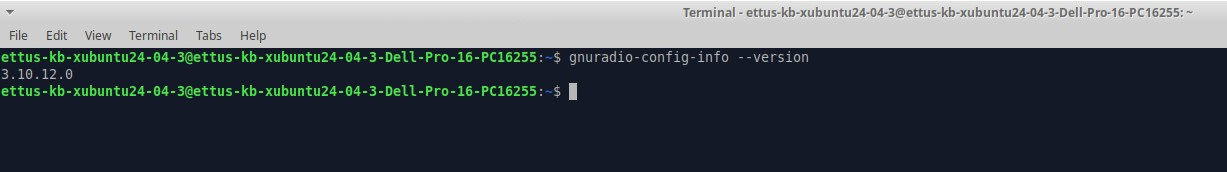
\includegraphics[width=0.75\linewidth]{latex/jpg_png/image_gnuradio-config-info --version.jpg}
\end{center}

\end{frame}